\documentclass[a4paper,UTF8]{article}
\usepackage{ctex}
\usepackage[margin=1.25in]{geometry}
\usepackage{color}
\usepackage{graphicx}
\usepackage{amssymb}
\usepackage{amsmath}
\usepackage{amsthm}
\usepackage{enumerate}
\usepackage{bm}
\usepackage{hyperref}
\numberwithin{equation}{section}
%\usepackage[thmmarks, amsmath, thref]{ntheorem}
\theoremstyle{definition}
\newtheorem*{solution}{Solution}
\newtheorem*{prove}{Proof}
\usepackage{multirow}

\renewcommand\refname{Reference}
\renewcommand\figurename{Figure}

%--

%--
\begin{document}
\title{机器学习导论\\
习题四}
\author{141242006, 袁帅, 141242006@smail.nju.edu.cn}
\maketitle
\vspace{0.08in}
\section{\textbf{[20pts]} Reading Materials on CNN}
卷积神经网络(Convolution Neural Network,简称CNN)是一类具有特殊结构的神经网络,在深度学习的发展中具有里程碑式的意义。其中,Hinton于2012年提出的\href{https://en.wikipedia.org/wiki/AlexNet}{AlexNet}可以说是深度神经网络在计算机视觉问题上一次重大的突破。

关于AlexNet的具体技术细节总结在经典文章\href{https://papers.nips.cc/paper/4824-imagenet-classification-with-deep-convolutional-neural-networks}{“ImageNet Classification with Deep Convolutional Neural Networks”}, by Alex Krizhevsky, Ilya Sutskever and Geoffrey E. Hinton in NIPS'12,目前已逾万次引用。在这篇文章中,它提出使用ReLU作为激活函数,并创新性地使用GPU对运算进行加速。请仔细阅读该论文,并回答下列问题(请用1-2句话简要回答每个小问题,中英文均可)。

\begin{enumerate}[(a)]
\item \textbf{[5pts]} Describe your understanding of how ReLU helps its success? And, how do the GPUs help out?
\item \textbf{[5pts]} Using the average of predictions from several networks help reduce the error rates. Why?
\item \textbf{[5pts]} Where is the dropout technique applied? How does it help? And what is the cost of using dropout?
\item \textbf{[5pts]} How many parameters are there in AlexNet? Why the dataset size(1.2 million) is important for the success of AlexNet?
\end{enumerate}

关于CNN,推荐阅读一份非常优秀的学习材料,由南京大学计算机系吴建鑫教授\footnote{吴建鑫教授主页链接为\url{cs.nju.edu.cn/wujx}}所编写的讲义Introduction to Convolutional Neural Networks\footnote{由此链接可访问讲义\url{https://cs.nju.edu.cn/wujx/paper/CNN.pdf}},本题目为此讲义的Exercise-5,已获得吴建鑫老师授权使用。
~\\
~\\
\begin{solution}
\item[(a)] ReLU is used as the neuron's activation function. The advantages of ReLU could be summarized as: (i) to provide non-saturating nonlinearity and hence to make the model fit complicated functions better; (ii) to speed up the training session; (iii) to prevent gradient from vanishing in back-propagation under the SGD scheme.

GPUs facilitate the training session by optimizing computational costs of 2D convolution. Specifically, the layer training memory are distributed separately on two GPUs and the GPUs only communicate on certain layers.

\item[(b)] Averaging predictions from several networks is a perfect example of \textit{Ensemble Learning}. In AlexNet, various random factors are introduced in the model by random initiations and random dropout processes, so the learning result could be diverse. By averaging random variables, we can make occasional errors less critical.

\item[(c)] Dropout is applied in the first two fully-connected layers by setting to zero the output of each hidden neuron with probability 0.5. This technique reduces complex co-adaptations of neurons, forces neurons to learn robust features and therefore reduces overfitting. Nevertheless, the running time with dropout technique is doubled because more iterations are required to converge.

\item[(d)] This model's parameters include convolutional kernels, neuron biases and fully-connected weights. The number of parameters in AlexNet is estimated as around 60 million. A large dataset is necessary for complicated models to reduce overfitting.

\end{solution}

\section{[20pts] Kernel Functions}
\begin{enumerate}[(1)]
\item 试通过定义证明以下函数都是一个合法的核函数:
	\begin{enumerate}[(i)]
	\item \textbf{[5pts]} 多项式核: $\kappa(\mathbf{x}_i,\mathbf{x}_j) = (\mathbf{x}_i^\mathrm{T}\mathbf{x}_j)^d$;
	\item \textbf{[10pts]} 高斯核:$\kappa(\mathbf{x}_i,\mathbf{x}_j) = \exp(-\frac{\lVert \mathbf{x}_i - \mathbf{x}_j \rVert^2}{2\sigma^2})$, 其中$\sigma > 0$.
	\end{enumerate}
\item \textbf{[5pts]} 试证明$\kappa(\mathbf{x}_i,\mathbf{x}_j)=\frac{1}{1+e^{-\mathbf{x}_i^T\mathbf{x}_j}}$不是合法的核函数。
\end{enumerate}
\begin{prove}
\item{(1).} By definition, in order to prove the kernel function's validity, we try to find a mapping $\bm{\phi}: \mathbb{R}^n\mapsto \mathbb{R}^m$, such that $\kappa(\bm{x}, \bm{y})=\bm{\phi}(\bm{x})^T\bm{\phi}(\bm{y})$. 

\paragraph{Polynomial kernel: } Wikipedia\cite{ref: wiki_poly_kernel} gives a specific proof for the case $d=2$. To expand that proof, for any vector $\bm{x}=(x_1,x_2,\cdots, x_n)^T$ and $\bm{y}=(y_1,y_2,\cdots, y_n)^T$, consider
\begin{equation}\label{multiexpand}
\kappa(\bm{x},\bm{y})=(\bm{x}^\mathrm{T}\bm{y})^d=(\sum_{i=1}^nx_iy_i)^d=\sum_{\substack{0\leq t_1,t_2,\cdots,t_n\leq d \\ t_1+t_2+\cdots+t_n=d}}\left[\begin{pmatrix}d\\t_1,t_2,\cdots,t_n\end{pmatrix}\cdot\prod_{j=1}^n(x_jy_j)^{t_j}\right],
\end{equation}
in which $\begin{pmatrix}d\\t_1,t_2,\cdots,t_n\end{pmatrix}=\begin{pmatrix}d\\t_1\end{pmatrix}\begin{pmatrix}d-t_1\\t_2\end{pmatrix}\begin{pmatrix}d-t_1-t_2\\t_3\end{pmatrix}\cdots\begin{pmatrix}d-t_1-\cdots-t_{n-1}\\t_n\end{pmatrix}$ is the \textit{multinomial coefficient}. Suppose $\bm{t}=(t_1,t_2,\cdots,t_n)^\mathrm{T}$ is an assignment such that $0\leq t_i\leq d$ for all $i\in\{1,2,\cdots,n\}$ and $\sum_{i=1}^n t_i=d$. We can define function
\begin{equation}
f(\bm{x}, \bm{t})=\sqrt{\begin{pmatrix}d\\t_1,t_2,\cdots,t_n\end{pmatrix}}\cdot\prod_{i=1}^n x_i^{t_i},
\end{equation}
so that $f(\bm{x},\bm{t})f(\bm{y},\bm{t})$ is equivalent to each term in the summation of Eq.(\ref{multiexpand}). In fact, numerous ($m=\begin{pmatrix}d+n-1\\d\end{pmatrix}$ in total) distinct $\bm{t}$ can be found, which can be enumerated as $\bm{t}^{(1)}, \bm{t}^{(2)}, \cdots, \bm{t}^{(m)}$. Thus we can define
\begin{equation}
\bm{\phi}_{\textbf{poly}}(\bm{x})=\left(f(\bm{x},\bm{t}^{(1)}), f(\bm{x},\bm{t}^{(2)}), ..., f(\bm{x},\bm{t}^{(n)})\right)^\mathrm{T},
\end{equation}
so that
\begin{eqnarray}
\bm{\phi}_{\textbf{poly}}(\bm{x})^\mathrm{T}\bm{\phi}_{\textbf{poly}}(\bm{y})&=&\sum_{i=1}^mf(\bm{x},\bm{t}^{(i)})f(\bm{y},\bm{t}^{(i)})=\sum_{i=1}^m\left[\begin{pmatrix}d\\t_1^{(i)},t_2^{(i)},\cdots,t_n^{(i)}\end{pmatrix}\cdot\prod_{j=1}^n(x_jy_j)^{t_j^{(i)}}\right]\nonumber\\
&=&\sum_{\substack{0\leq t_1,t_2,\cdots,t_n\leq d \\ t_1+t_2+\cdots+t_n=d}}\left[\begin{pmatrix}d\\t_1,t_2,\cdots,t_n\end{pmatrix}\cdot\prod_{j=1}^n(x_jy_j)^{t_j}\right]=\kappa(\bm{x},\bm{y}).
\end{eqnarray}
Therefore, the polynomial kernel function can be construed as a dot product in a $\begin{pmatrix}d+n-1\\d\end{pmatrix}$-dimensional space, so the corresponding polynomial kernel function is valid.

\paragraph{RBF kernel: } According to \cite{ref: mathb}, we can taylor expand the kernel function as
\begin{eqnarray}
\kappa(\bm{x},\bm{y})&=&\exp(-\frac{\lVert \bm{x}-\bm{y}\rVert^2}{2\sigma^2})=\exp(-\frac{\bm{x}^\mathrm{T}\bm{x}}{2\sigma^2})\cdot\exp(\frac{\bm{x}^\mathrm{T}\bm{y}}{\sigma^2})\cdot\exp(-\frac{\bm{y}^\mathrm{T}\bm{y}}{2\sigma^2})\nonumber\\
&=&\exp(-\frac{\bm{x}^\mathrm{T}\bm{x}}{2\sigma^2})\cdot\sum_{d=0}^{\infty}\frac{(\bm{x}^\mathrm{T}\bm{y})^d}{d!\cdot\sigma^{2d}} \cdot\exp(-\frac{\bm{y}^\mathrm{T}\bm{y}}{2\sigma^2})\nonumber\\
&=&\sum_{d=0}^{\infty}\frac{\exp(-\frac{\bm{x}^\mathrm{T}\bm{x}}{2\sigma^2})}{\sqrt{d!}\sigma^{d}}\cdot(\bm{x}^\mathrm{T}\bm{y})^d\cdot\frac{\exp(-\frac{\bm{y}^\mathrm{T}\bm{y}}{2\sigma^2})}{\sqrt{d!}\sigma^{d}}\nonumber\\
&=&\sum_{d=0}^{\infty}\frac{\exp(-\frac{\bm{x}^\mathrm{T}\bm{x}}{2\sigma^2})}{\sqrt{d!}\sigma^{d}}\cdot\bm{\phi}_{\textbf{poly}}(\bm{x}, d)^\mathrm{T}\bm{\phi}_{\textbf{poly}}(\bm{y},d)\cdot\frac{\exp(-\frac{\bm{y}^\mathrm{T}\bm{y}}{2\sigma^2})}{\sqrt{d!}\sigma^{d}}.
\end{eqnarray}
Hence, by defining vector function $\bm{g}(\bm{x},d)=\frac{\exp(-\frac{\bm{x}^\mathrm{T}\bm{x}}{2\sigma^2})}{\sqrt{d!}\sigma^{d}}\cdot\bm{\phi}_{\textbf{poly}}(\bm{x},d)$,\footnote{When $d=0$, $\bm{\phi}_{\textbf{poly}}(\bm{x},d)$ is the scalar 1; otherwise, it is the mapping for polynomial kernel with parameter $d$.} we have mapping $\bm{\phi}_{\textbf{rbf}}: \mathbb{R}^n\mapsto\mathbb{R}^{\infty}$, which concatenates all $\bm{g}(\bm{x},d)$, i.e.
\begin{equation}
\bm{\phi}_{\textbf{rbf}}(\bm{x})=(\bm{g}(\bm{x},0)^\mathrm{T}, \bm{g}(\bm{x},1)^\mathrm{T}, \bm{g}(\bm{x},2)^\mathrm{T}, \cdots)^\mathrm{T},
\end{equation}
so that 
\begin{eqnarray}
\bm{\phi}_{\textbf{rbf}}(\bm{x})^\mathrm{T}\bm{\phi}_{\textbf{rbf}}(\bm{y})&=&\sum_{d=0}^{\infty}\bm{g}(\bm{x},d)^\mathrm{T}\bm{g}(\bm{y},d)\nonumber\\
&=&\sum_{d=0}^{\infty}\frac{\exp(-\frac{\bm{x}^\mathrm{T}\bm{x}}{2\sigma^2})}{\sqrt{d!}\sigma^{d}}\cdot\bm{\phi}_{\textbf{poly}}(\bm{x}, d)^\mathrm{T}\bm{\phi}_{\textbf{poly}}(\bm{y},d)\cdot\frac{\exp(-\frac{\bm{y}^\mathrm{T}\bm{y}}{2\sigma^2})}{\sqrt{d!}\sigma^{d}}\nonumber\\
&=&\kappa(\bm{x},\bm{y}).
\end{eqnarray}
Therefore, the RBF kernel function can be rewritten as a dot product in an infinite-dimensional space, so the corresponding kernel function is valid.

\item[(2).] A counter-example could be raised to disprove the kernel function's validity: consider scalar (unidimensional vector) $x_1=\frac{1}{2}$ and $x_2=10$. The kernel matrix
\begin{equation}
\bm{K}=\left[\begin{array}{ll}\kappa(x_1,x_1)&\kappa(x_1,x_2)\\\kappa(x_2,x_1)&\kappa(x_2,x_2)\end{array}\right]=\left[\begin{array}{ll}\frac{1}{1+\exp(-\frac{1}{4})}&\frac{1}{1+\exp(-5)}\\\frac{1}{1+\exp(-5)}&\frac{1}{1+\exp(-100)}\end{array}\right].
\end{equation}
For non-zero vector $\bm{w}=(-\frac{1}{1+\exp(-5)}, \frac{1}{1+\exp(-\frac{1}{4})})$, the quadratic form $\bm{w}^\mathrm{T}\bm{K}\bm{w}\\=\frac{1}{1+\exp(-\frac{1}{4})}(-\frac{1}{1+\exp(-5)})^2-2\frac{1}{1+\exp(-5)}\cdot\frac{1}{1+\exp(-5)}\cdot\frac{1}{1+\exp(-\frac{1}{4})}+\frac{1}{1+\exp(-100)}(\frac{1}{1+\exp(-\frac{1}{4})})^2\\=\frac{1}{1+\exp(-\frac{1}{4})}\left[\frac{1}{1+\exp(-100)}\cdot\frac{1}{1+\exp(-\frac{1}{4})}-(\frac{1}{1+\exp(-5)})^2\right]<0$. Therefore, $\bm{K}$ is not positive semi-definite, and the kernel function is not valid.
\qed
~\\
\end{prove}

\section{[25pts] SVM with Weighted Penalty}
考虑标准的SVM优化问题如下(即课本公式(6.35)),
\begin{equation}
\label{eq-svm}
\begin{split}
\min_{\mathbf{w},b,\xi_i}& \quad \frac{1}{2} \lVert \mathbf{w} \rVert^2 + C\sum_{i=1}^m\xi_i\\
\text{s.t.}&  \quad y_i(\mathbf{w}^\mathrm{T}\mathbf{x}_i + b)\geq 1-\xi_i\\
& \quad \xi_i \geq 0, i = 1,2,\cdots,m.
\end{split}
\end{equation}

注意到,在\eqref{eq-svm}中,对于正例和负例,其在目标函数中分类错误的“惩罚”是相同的。在实际场景中,很多时候正例和负例错分的“惩罚”代价是不同的,比如考虑癌症诊断,将一个确实患有癌症的人误分类为健康人,以及将健康人误分类为患有癌症,产生的错误影响以及代价不应该认为是等同的。

现在,我们希望对负例分类错误的样本(即false positive)施加$k>0$倍于正例中被分错的样本的“惩罚”。对于此类场景下,

(1) \textbf{[10pts]} 请给出相应的SVM优化问题;

(2) \textbf{[15pts]} 请给出相应的对偶问题,要求详细的推导步骤,尤其是如KKT条件等。
\begin{solution}
\item[(1).]
Similarly, we introduce slack variable $\xi_i$ to measure the loss. In the standard form, both false positive and false negative cases have the same contribution to total loss; in this problem, we distinguish these cases and assign different penalties separately. Specifically, we can write each \textit{penalty} as
\begin{eqnarray}\label{ell}
\ell_i&=&\mathbb{I}(y_i=1)\cdot C\xi_i+\mathbb{I}(y_i=-1)\cdot kC\xi_i\nonumber\\
&=&\frac{y_i+1}{2}\cdot C\xi_i+\frac{-y_i+1}{2}\cdot kC\xi_i\nonumber\\
&=&\frac{C}{2}\xi_i[k+1+(1-k)y_i].
\end{eqnarray}
Note that in Eq.(\ref{ell}), the denominator 2 can be absorbed by constant $C$. Therefore, the formalized optimization problem could be presented as
\begin{equation}
\label{mod-svm}
\begin{split}
\min_{\bm{w},b,\bm{\xi}}& \quad \frac{1}{2} \lVert \mathbf{w} \rVert^2 + C\sum_{i=1}^m\xi_i[k+1+(1-k)y_i]\\
\text{s.t.}&  \quad y_i(\bm{w}^\mathrm{T}\bm{x}_i + b)\geq 1-\xi_i\\
& \quad \xi_i \geq 0, \  i = 1,2,\cdots,m.
\end{split}
\end{equation}

\item[(2).] The Lagrange function is
\begin{equation}
L(\bm{w}, b, \bm{\xi}, \bm{\lambda}, \bm{\mu})=\frac{1}{2} \lVert \mathbf{w} \rVert^2 + C\sum_{i=1}^m\xi_i[k+1+(1-k)y_i]+\sum_{i=1}^{m}\lambda_i(1-\xi_i-y_i(\bm{w}^\mathrm{T}\bm{x}_i+b))-\sum_{i=1}^m\mu_i\xi_i.
\end{equation}
By setting derivatives $\frac{\partial L}{\partial \bm{w}}=0$, $\frac{\partial L}{\partial b}=0$ and $\frac{\partial L}{\partial \bm{\xi}}=0$, we obtain
\begin{eqnarray}
\bm{w}&=&\sum_{i=1}^m\lambda_iy_i\bm{x}_i, \label{p1}\\
\sum_{i=1}^m\lambda_iy_i&=&0, \label{p2}\\
\lambda_i+\mu_i&=&C[k+1+(1-k)y_i]. \label{p3}
\end{eqnarray}
Plugging back Eq.(\ref{p1}), Eq.(\ref{p2}) and Eq.(\ref{p3}), we get the dual problem as
\begin{equation}
\label{mod-svm}
\begin{split}
\max_{\bm{\lambda}}& \quad \sum_{i=1}^m\lambda_i-\frac{1}{2}\sum_{i=1}^m\sum_{j=1}^m\lambda_i\lambda_jy_iy_j\bm{x}_i^\mathrm{T}\bm{x}_j\\
\text{s.t.}&  \quad \sum_{i=1}^m\lambda_iy_i=0,\\
& \quad 0\leq\lambda_i\leq C[k+1+(1-k)y_i], \  i = 1,2,\cdots,m.
\end{split}
\end{equation}
and the corresponding KKT conditions are:  for each $i= 1,2,\cdots,m$,
\begin{equation}
\left\{
\begin{array}{l}
\lambda_i\geq 0,\ \ \mu_i\geq 0, \\
1-\xi_i-y_i(\bm{w}^\mathrm{T}\bm{x}_i+b)\leq 0, \\
\lambda_i(1-\xi_i-y_i(\bm{w}^\mathrm{T}\bm{x}_i+b))=0,\\
\xi_i\geq 0, \ \ \mu_i\xi_i=0.
\end{array}
\right.
\end{equation}
~\\
\end{solution}

\section{[35pts] SVM in Practice - LIBSVM} 
支持向量机(Support Vector Machine,简称SVM)是在工程和科研都非常常用的分类学习算法。有非常成熟的软件包实现了不同形式SVM的高效求解,这里比较著名且常用的如LIBSVM\footnote{LIBSVM主页课参见链接:\url{https://www.csie.ntu.edu.tw/~cjlin/libsvm/}}。

(1) \textbf{[20pts]} 调用库进行SVM的训练,但是用你自己编写的预测函数作出预测。

(2) \textbf{[10pts]} 借助我们提供的可视化代码,简要了解绘图工具的使用,通过可视化增进对SVM各项参数的理解。详细编程题指南请参见链接:\url{http://lamda.nju.edu.cn/ml2017/PS4/ML4_programming.html}. 

(3) \textbf{[5pts]} 在完成上述实践任务之后,你对SVM及核函数技巧有什么新的认识吗?请简要谈谈。

\begin{solution}
\begin{figure}[htbp] %  figure placement: here, top, bottom, or page
   \centering
   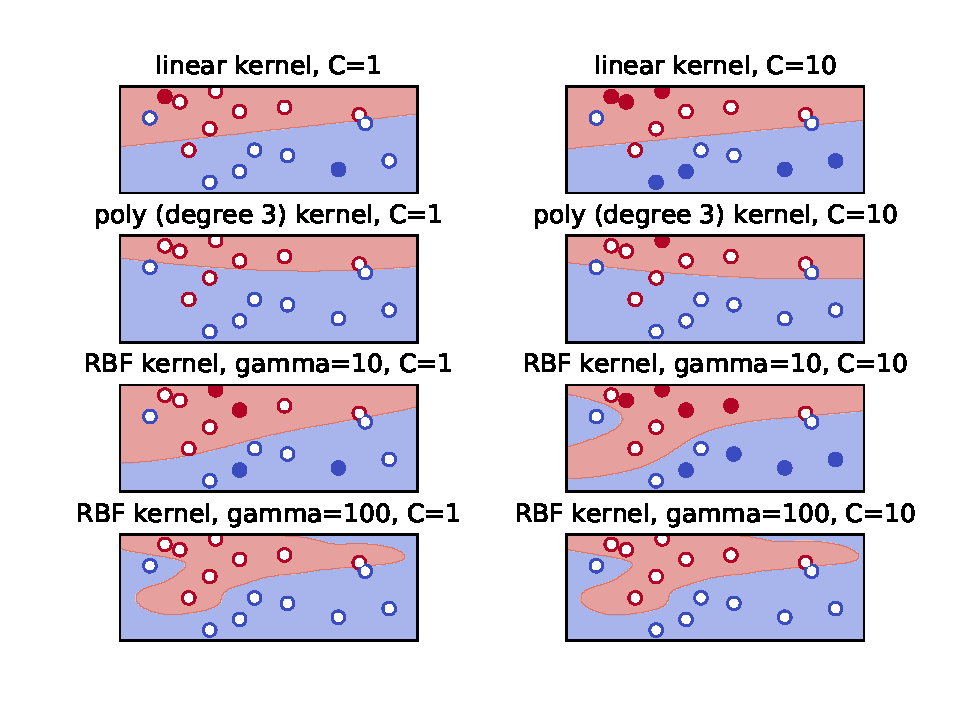
\includegraphics[width=5in]{figure.pdf} 
\end{figure}
Above are the results of six different kernel configurations on the demo dataset. All support vectors are marked by a white dot. To illustrate how different kernels work in SVM, I tried some more interesting data points, which are shown in Fig.(\ref{xor}) and Fig.(\ref{ring}).

\begin{figure}[htbp] %  figure placement: here, top, bottom, or page
\begin{minipage}[t]{0.48\linewidth}
   \centering
   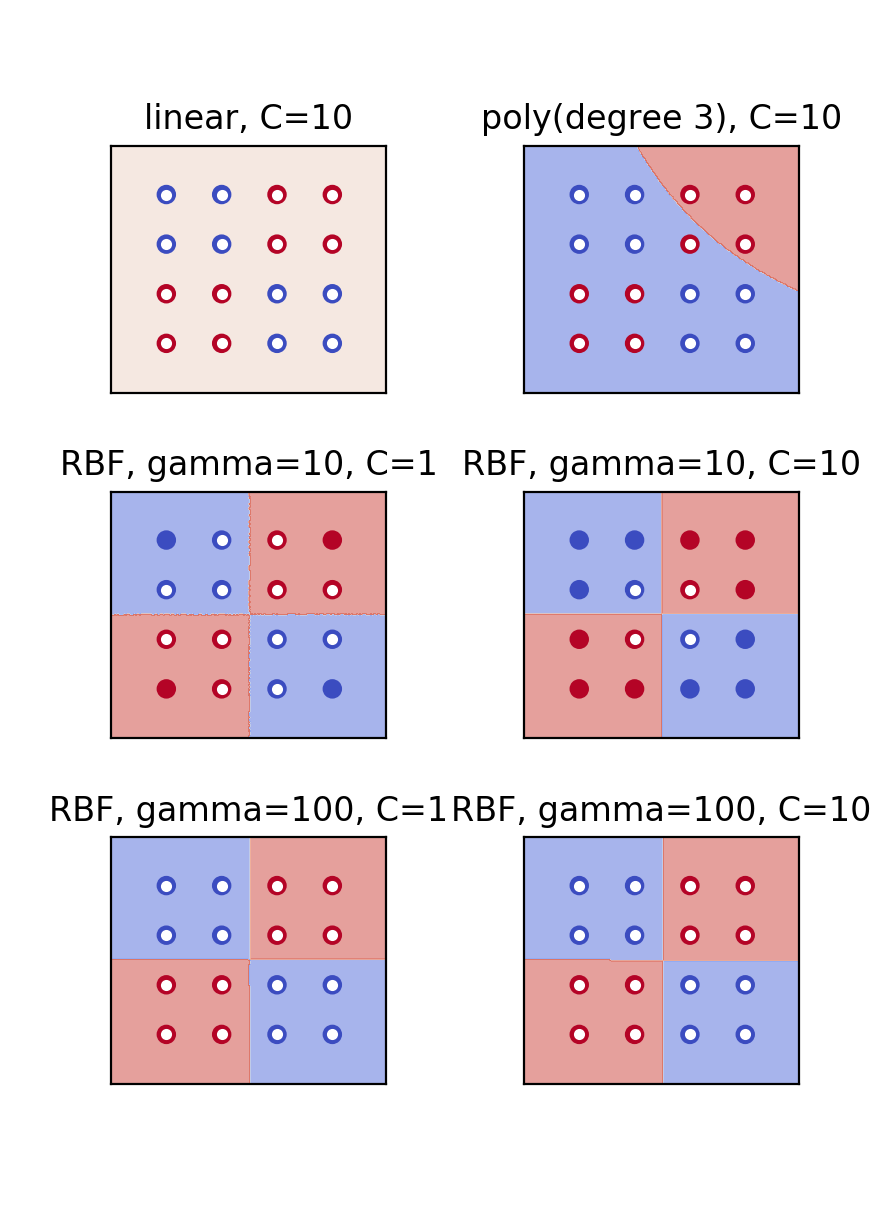
\includegraphics[width=2.4in]{fig_1.png}
   \caption{The XOR problem}
   \label{xor}
\end{minipage}
\begin{minipage}[t]{0.48\linewidth}
   \centering
   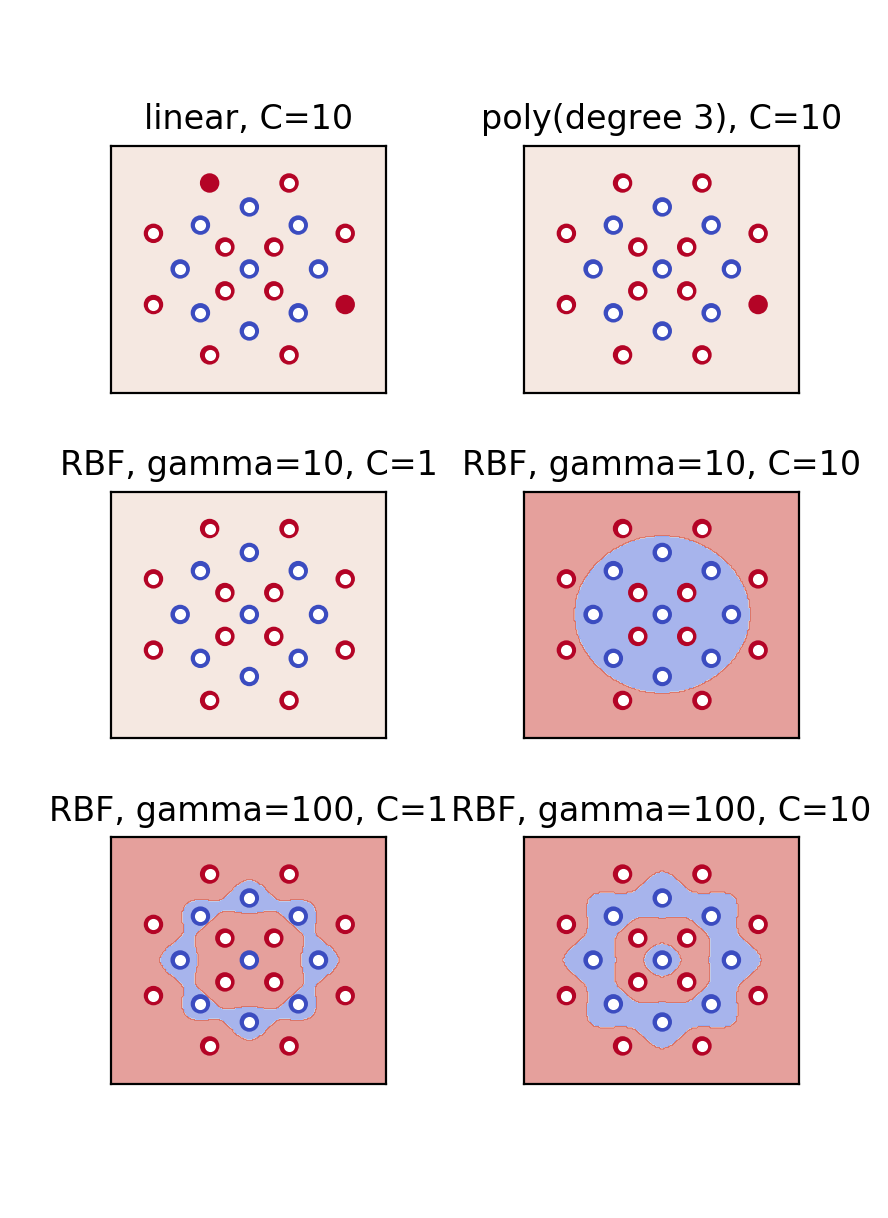
\includegraphics[width=2.4in]{fig_2.png}
   \caption{The embedded rings problem}
   \label{ring}
\end{minipage}
\end{figure}

In the XOR problem (Fig.(\ref{xor})), data from the same class are put on one of the two diagonal areas. In this case, linear kernel is not functioning: it simply interpret all data points as positive instances, so the visualization method based on contour doesn't work. The cubic polynomial kernel can only deal with one part of the positive cases, while leaving the other half mistaken. Contrarily, RBF kernel works perfectly, dividing the input space into four distinct parts. Moreover, when we raise the parameters gamma and C in the RBF model, more data end up support vectors, embodying a growing model robustness.

In the embedded rings problem (Fig.(ref{ring})), certain data are distributed as a ring, and rings of different classes are embedded one another. In this complicated scenario, linear and polynomial kernels, just as we expected, doesn't work. A simple RBF kernel implementation also fails by labelling all data as the same class. When we try to increase the RBF parameters, the results are apparently getting better by separating the rings apart.

\end{solution}

\begin{thebibliography}{99}
\bibitem{ref: wiki_poly_kernel} Wikipedia. \textit{Polynomial kernel}. \\\url{https://en.wikipedia.org/wiki/Polynomial_kernel}.
\bibitem{ref: mathb} Matthew Bernstein. \textit{The Radical Basis Function Kernel}. University of Wisconsin - Madison. \url{http://pages.cs.wisc.edu/~matthewb/pages/notes/pdf/svms/RBFKernel.pdf}.
\bibitem{ref: svc} Scikit-learn. \textit{sklearn.svm.SVC Documentation}. \\
\url{http://scikit-learn.org/stable/modules/generated/sklearn.svm.SVC.html}.
\end{thebibliography}

\end{document}